\subsection{A chain reaction of constructions}\label{ssec:crossing}

The library of the package records known constructions with their provenance. The crossing network makes each of them a typed node and breeds new constructions from pairs of old ones, keeping an offspring only if it passes a check, so that every survivor is a checked construction that may seed the next generation. The experiment asks whether learning which crosses survive produces more new constructions than crossing at random.

\emph{The domain.} Let $f(n)$ be the largest $N$ such that every $2$-colouring of the subsets of $[n]=\{1,\dots,n\}$ has a monochromatic family of $N$ sets closed under union and intersection, Erd\H{o}s problem 1183 \cite{Blo1183}. A maximal chain has $n+1$ members and each of its colour classes is closed under both operations, so $f(n)\ge\lceil(n+1)/2\rceil$, and Chojecki proved $f(n)\le(3+o(1))\,n\log_{2}n$ \cite{Cho26}.\footnote{D.~Bhattacharjee, P.~Mandal and U.~Bhattacharya, \emph{Resolving Erd\H{o}s--Ulam monochromatic union-closed family conjectures}, arXiv:2610.02833v1 (2 October 2026), doi:10.48550/arXiv.2610.02833, with Lean~4 archive doi:10.5281/zenodo.23094057. The paper proves both conjectures of Erd\H{o}s and Ulam on families closed under union only, in Lean, bounds $f(n)$ by $O(n\log^{2}n)$ in its Theorem~1.4, and asks in its Question~9.3 whether $f(n)=O(n)$ and whether $f(n)=\lceil(n+1)/2\rceil$ for every $n$. Theorem~\ref{thm:fvalues} below gives the exact values for $n\le19$; the first question remains open.} A construction is a family of colourings, one for each $n$. Its genome is a typed expression tree: the leaves are words indexed by sizes (Thue--Morse, Rudin--Shapiro and Sturmian words, Legendre symbols modulo $5,7,11,13$, periodic words) and families of colourings (weighted sums of coordinates modulo $3$ and $4$, the parity of the least element), and the internal nodes are operations on words (sum modulo two, shift, reversal, dilation, interleaving) and on families (the level colouring of a word, sum modulo two, splitting the ground set, blowing up blocks, complementation, symmetrisation). Two parents breed by exchanging subtrees of the same type. The check computes the largest monochromatic sublattice $m(n)$ for $n=6,7,8,9$ with an exact search and keeps the offspring when $m(n)\le f(n)+1$; a colouring is new when its key, the colour profile of the sizes and of the elements, minimised over complementation of the sets and exchange of the colours, has not been met.

\emph{The arms.} Each arm breeds $40$ offspring in each of $6$ generations, over $5$ seeds, so every arm spends $1200$ checks. The \emph{network} draws parents by fitness, proposes eight typed crosses and evaluates the one ranked first by a logistic model of survival refitted every generation; \emph{select} draws parents by fitness and evaluates one typed cross; \emph{random} draws parents uniformly and evaluates one typed cross; \emph{blind} draws parents uniformly and crosses without regard to types. The experiment was run twice, freely and under a novelty rule that skips, before any check, an offspring whose colouring the arm has already evaluated (Fig.~\ref{fig:crossing}).

\begin{figure*}[t]
\centering
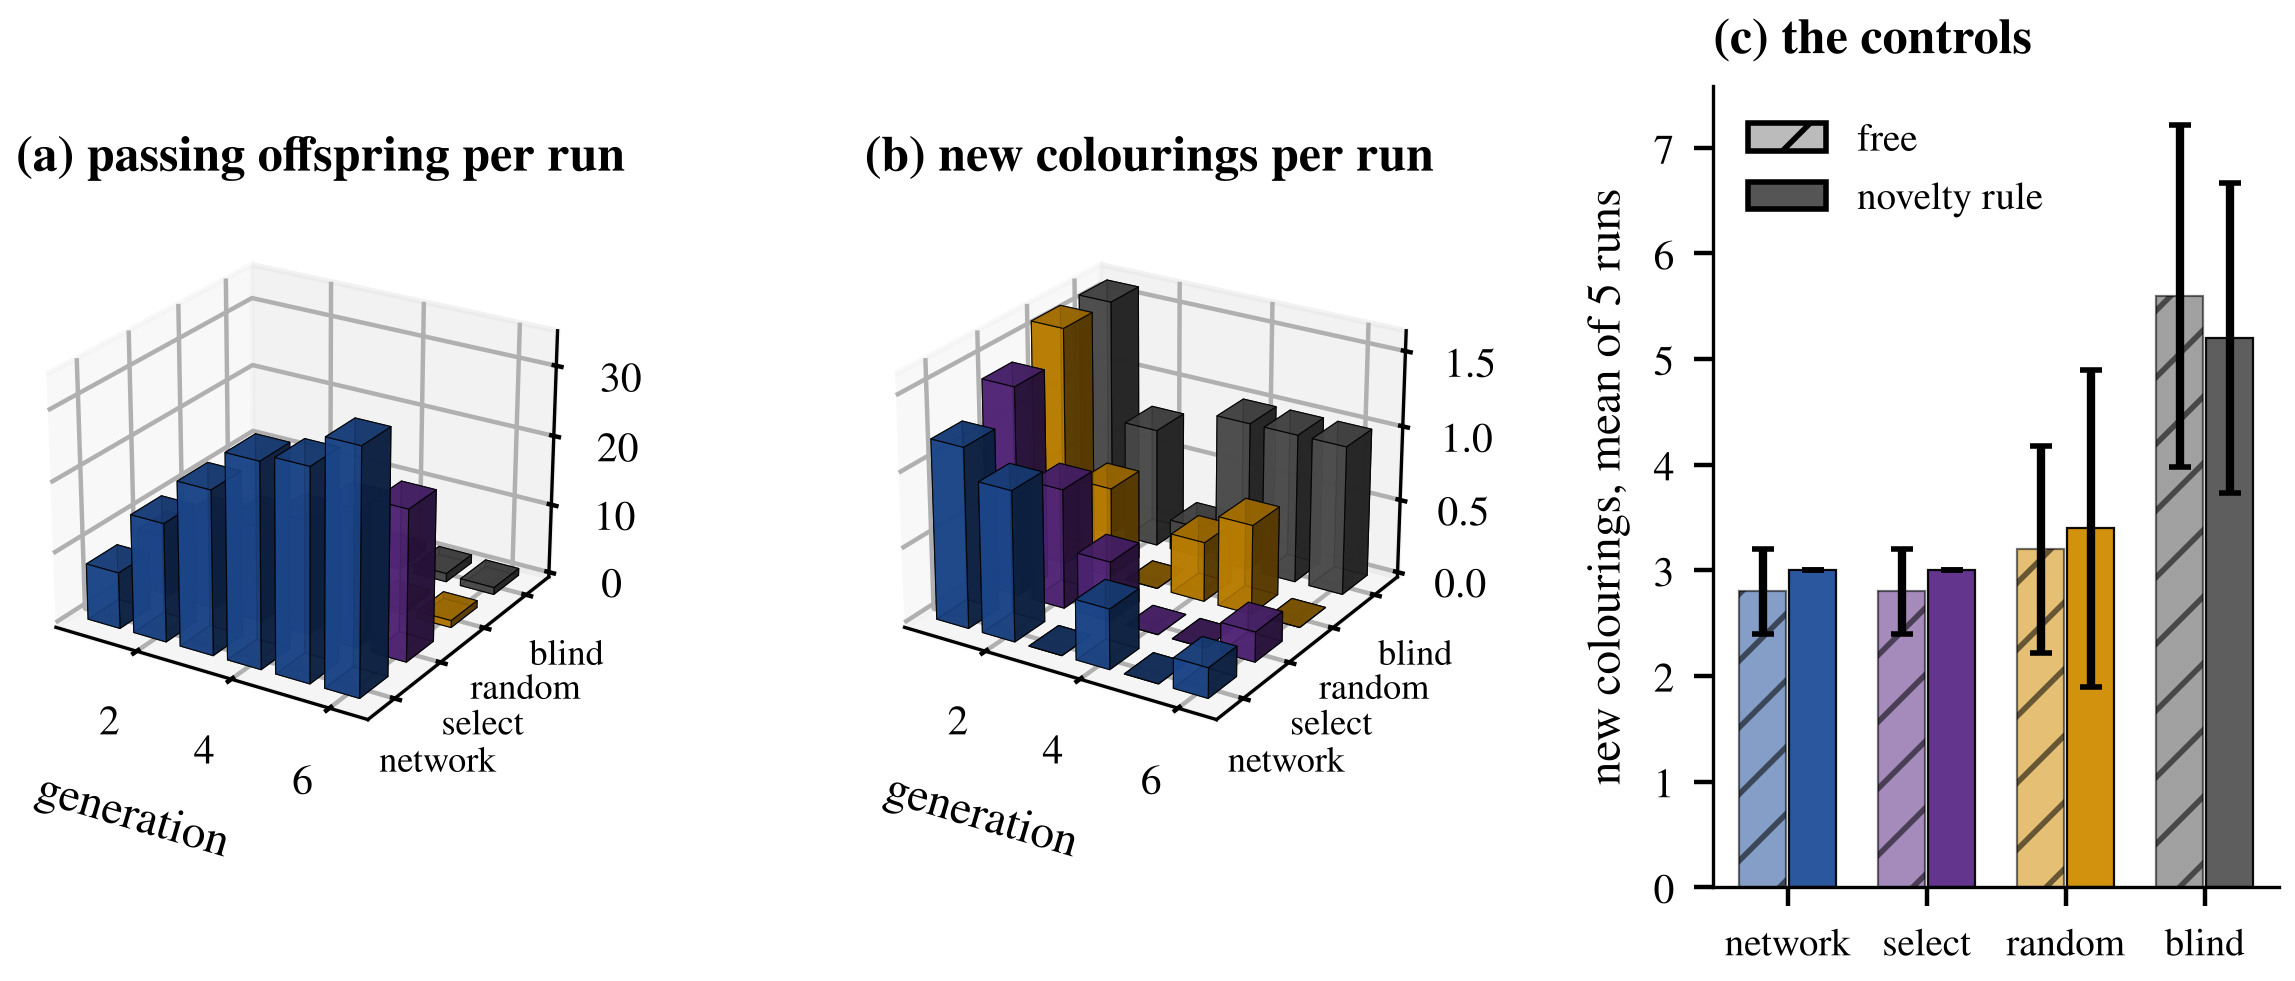
\includegraphics[width=0.98\textwidth]{figures/fig_crossing}
\caption{The crossing network against its controls on Erd\H{o}s problem 1183. (a) Offspring that pass the check, per generation, mean of five runs without the novelty rule. (b) Colourings not met before among them. (c) New colourings per run with and without the novelty rule, with one standard deviation. The network passes the most offspring and finds no more new colourings than the controls; the untyped arm finds the most.}
\label{fig:crossing}
\end{figure*}

\begin{table}[t]
\caption{The arms of the crossing network, five runs of $1200$ checks each. ``Pass'' is the share of offspring that pass the check; ``new'' is the number of new colourings per run (mean $\pm$ standard deviation) and ``optimal'' the number of them with $m(n)=f(n)$ for $n=6,\dots,9$. Ill-typed offspring are those of the blind arm that fail the typing.}
\label{tab:crossing}
\centering
\footnotesize
\setlength{\tabcolsep}{3.5pt}
\begin{tabular}{@{}lrrrr@{}}
\toprule
Arm & Pass & New & Optimal & Ill-typed \\
\midrule
\multicolumn{5}{@{}l}{\emph{free}}\\
network & $58.7\%$ & $2.8\pm0.4$ & $1.8$ & $0$ \\
select & $38.1\%$ & $2.8\pm0.4$ & $2.0$ & $0$ \\
random & $3.6\%$ & $3.2\pm1.0$ & $0.8$ & $0$ \\
blind & $2.7\%$ & $5.6\pm1.6$ & $1.6$ & $927$ \\
\multicolumn{5}{@{}l}{\emph{novelty rule}}\\
network & $1.3\%$ & $3.0\pm0.0$ & $2.0$ & $0$ \\
select & $1.4\%$ & $3.0\pm0.0$ & $2.0$ & $0$ \\
random & $1.4\%$ & $3.4\pm1.5$ & $1.0$ & $0$ \\
blind & $2.2\%$ & $5.2\pm1.5$ & $1.4$ & $1002$ \\
\bottomrule
\end{tabular}
\end{table}

\emph{The result} (Table~\ref{tab:crossing}). Without the novelty rule the network passes $58.7\%$ of its offspring against $3.6\%$ for random typed crossing, but almost all of them are colourings it has already found under another genome: it finds $2.8$ new colourings per run against $3.2$ for random crossing and $5.6$ for blind crossing. Under the novelty rule the pass rates fall to between $1.3\%$ and $2.2\%$ and the order of the new colourings is unchanged. The learned model therefore learns to repeat survivors, and it does not beat the random controls in the quantity that matters. Blind crossing does best because an untyped exchange occasionally grafts a family where a word was expected and so reaches combinations of the operations that typed crossing never proposes; the typing removes ill-formed genomes and, with them, part of the reachable set. None of the bred colourings improves a known value: the best, from the random arm, has $m(n)=7,7,8,8,9$ for $n=10,\dots,14$, which equals $f(n)$ at $n=11,13$ and exceeds it by one at $n=10,12,14$.

\emph{What did move the frontier} was a change of representation, not breeding. The optimal colourings found for $n=7,9,10$ by a counterexample-guided search over all colourings are level colourings, in which the colour of $S$ depends only on $|S|$; such a colouring is a word $c_{0}c_{1}\cdots c_{n}$, with colour classes $L_{0},L_{1}\subseteq\{0,\dots,n\}$. A \emph{weighted poset} is a finite poset $P$ with a map $w\colon P\to\{1,2,\dots\}$; $J(P)$ is its lattice of down-sets and $w(I)=\sum_{p\in I}w(p)$.

\begin{figure*}[t]
\centering
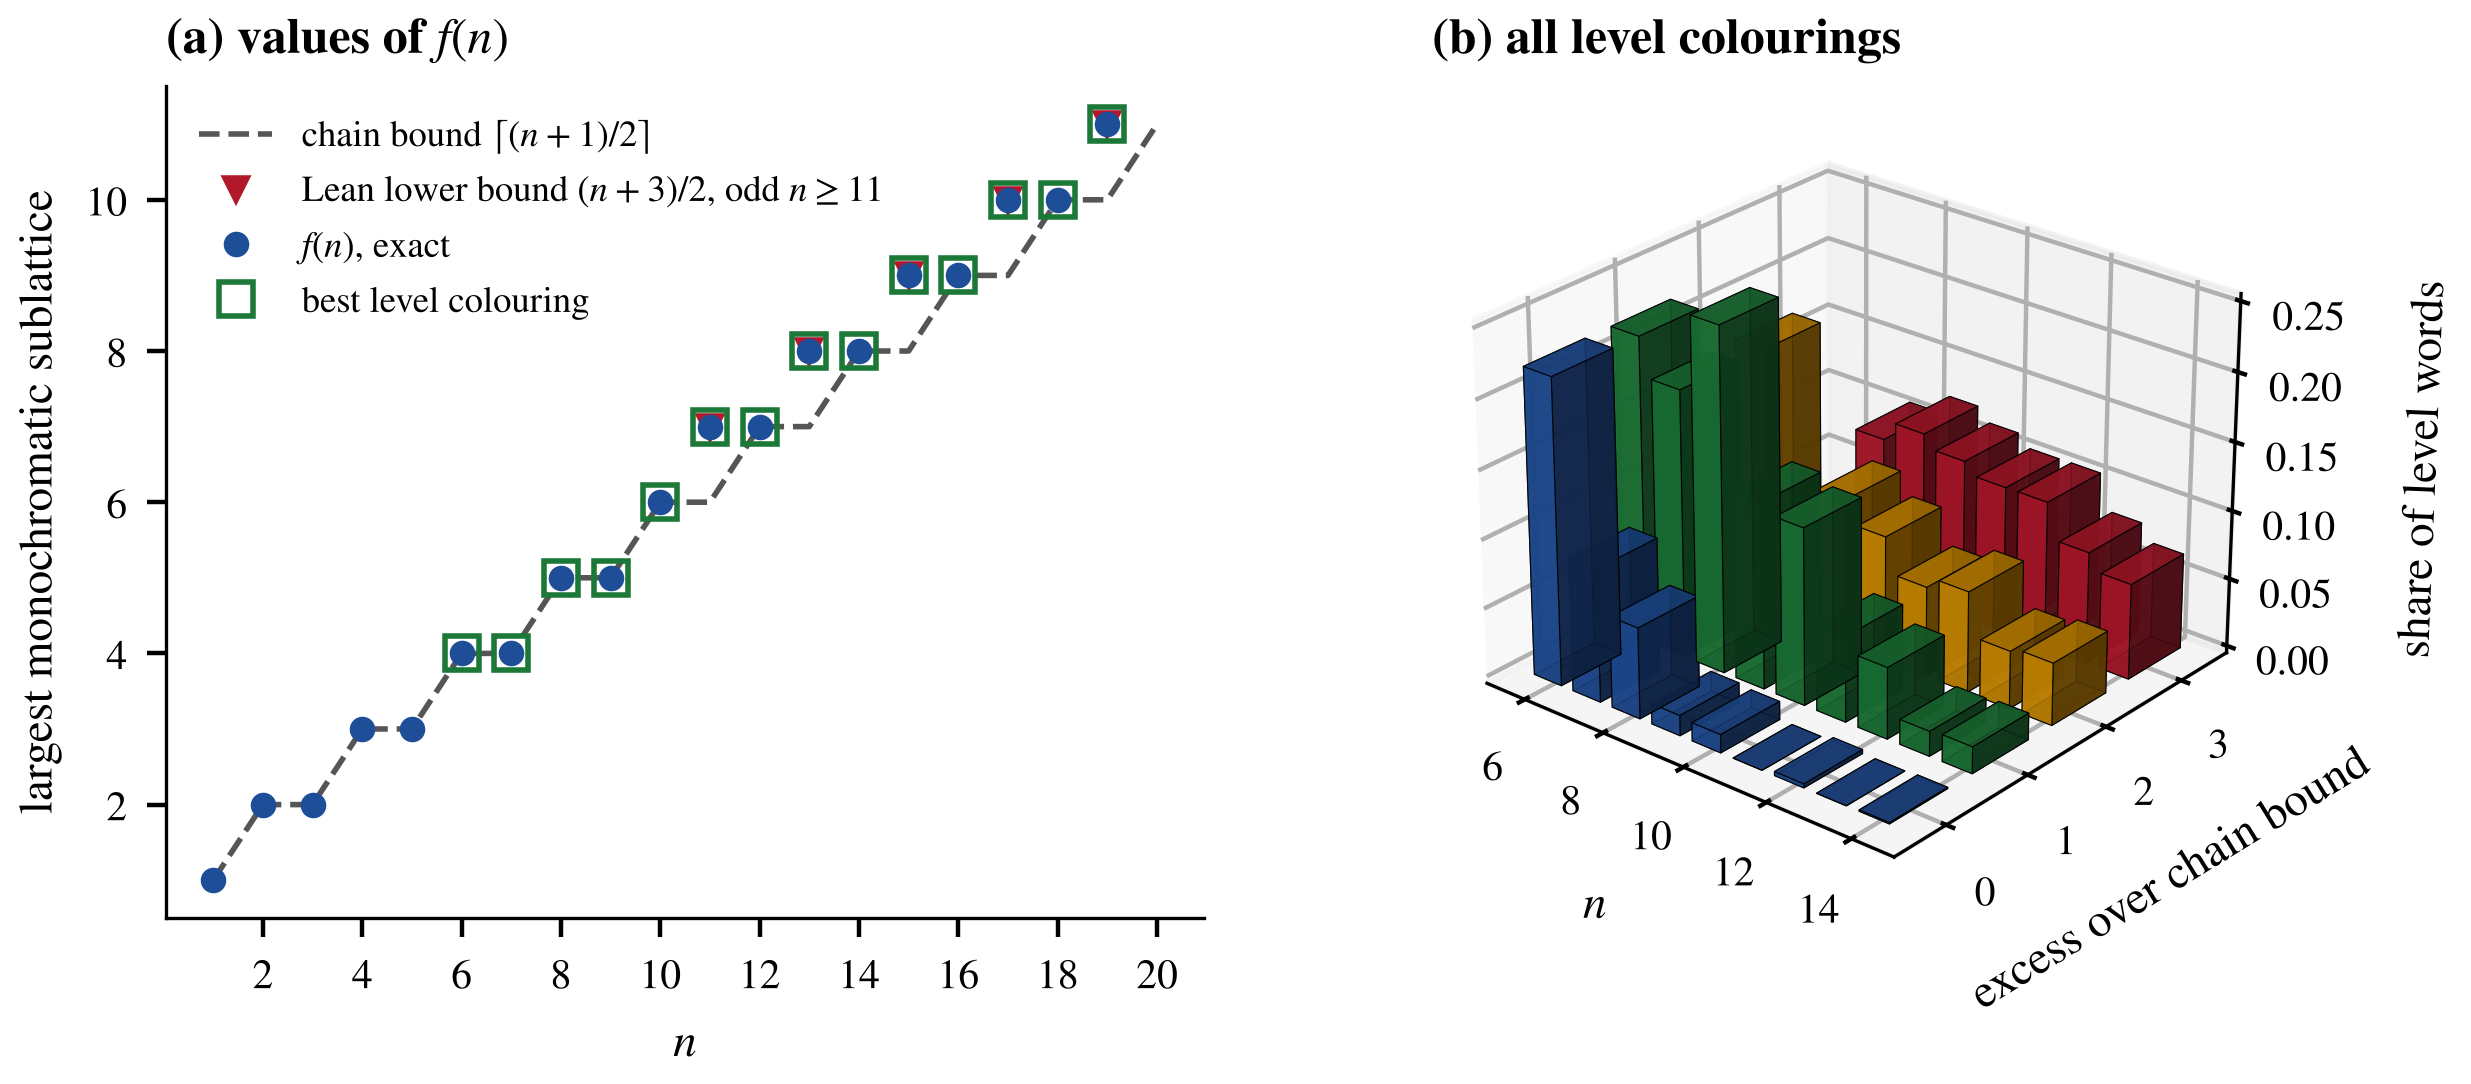
\includegraphics[width=0.98\textwidth]{figures/fig_sublattice}
\caption{Monochromatic sublattices of colourings of $2^{[n]}$. (a) The exact values of $f(n)$ for $n\le19$ (Theorem~\ref{thm:fvalues}), the chain bound $\lceil(n+1)/2\rceil$, the Lean lower bound $(n+3)/2$ for odd $n\ge11$ \cite{ORf1183}, and the best level colouring, which attains $f(n)$ for every $n\le19$. (b) The distribution of the largest monochromatic sublattice over all level colourings for $6\le n\le14$, by its excess over the chain bound; the share of words that attain the bound falls quickly with $n$, and from $n=11$ on no odd word does.}
\label{fig:sublattice}
\end{figure*}

\begin{lemma}\label{lem:levelposet}
A level colouring has a monochromatic sublattice of colour class $L$ with $N$ members if and only if there are a weighted poset $(P,w)$ and an integer $t\ge0$ with $t+w(P)\le n$, $|J(P)|=N$ and $t+w(I)\in L$ for every $I\in J(P)$.
\end{lemma}

\begin{proof}
Let $D$ be a sublattice of $2^{[n]}$ with $N$ members whose sizes lie in $L$. It is a finite distributive lattice, so by Birkhoff's theorem it is isomorphic to $J(P)$ for the poset $P$ of its join-irreducible members, by the map that sends $A\in D$ to the set of join-irreducibles below it. The function $A\mapsto|A|$ is strictly increasing on $D$ and modular, since $|A\cup B|+|A\cap B|=|A|+|B|$. Write $p_{*}$ for the unique lower cover of a join-irreducible $p$ and $w(p)=|p|-|p_{*}|\ge1$. If $I$ is a down-set and $p$ a minimal element of $P\setminus I$, then $I\cup\{p\}$ is the join of $I$ and the principal down-set of $p$, and their meet is that principal down-set without $p$, which corresponds to $p_{*}$, so modularity gives $|I\cup\{p\}|=|I|+w(p)$; induction along a maximal chain of down-sets gives $|A|=t+w(I)$ with $t=|\min D|$, and $t+w(P)=|\max D|\le n$. Conversely, given $(P,w,t)$, choose disjoint sets $T$ and $B_{p}$ $(p\in P)$ in $[n]$ with $|T|=t$ and $|B_{p}|=w(p)$; the map $I\mapsto T\cup\bigcup_{p\in I}B_{p}$ is injective, carries unions and intersections of down-sets to unions and intersections of sets, and gives $I$ the size $t+w(I)\in L$.
\end{proof}

The lemma replaces the search over sublattices of $2^{[n]}$ by a search over weighted posets, which is small: the elements of $P$ are added in the order of the weights of their principal down-sets, each new element is placed above a down-set already built and creates the down-sets $I\cup\{p\}$ for every $I$ above that one, and a branch stops as soon as a new size leaves $L$. On $120$ random level colourings with $3\le n\le9$ the poset search and the general search agree on the largest monochromatic sublattice in every case, and on $30$ at $n=10$ they agree on every value below the cap of the poset search. A grid version, for colourings that depend on the sizes of $S$ in the blocks of a fixed partition of $[n]$, holds with weights in $\NN^{k}\setminus\{0\}$ by the same proof.

\begin{theorem}\label{thm:fvalues}
For $1\le n\le 19$,
\[
f(n)=\begin{cases}\lceil (n+1)/2\rceil & \text{if } n\le 10 \text{ or } n \text{ is even},\\[2pt] (n+3)/2 & \text{if } n\ge 11 \text{ is odd},\end{cases}
\]
and $f(20)\in\{11,12\}$. For $11\le n\le19$ the bound is attained by the level colouring of the word in the table below.
\begin{center}\small
\begin{tabular}{@{}rl@{\qquad}rl@{}}
$n$ & word $c_{0}\cdots c_{n}$ & $n$ & word $c_{0}\cdots c_{n}$\\
\midrule
$11$ & \texttt{110111001000} & $16$ & \texttt{10011001011100100}\\
$12$ & \texttt{1010011100100} & $17$ & \texttt{110100111001101000}\\
$13$ & \texttt{10111001101000} & $18$ & \texttt{0011001011100110100}\\
$14$ & \texttt{011010011100100} & $19$ & \texttt{00110010111000101101}\\
$15$ & \texttt{1100111010011000} & &
\end{tabular}
\end{center}
\end{theorem}

\begin{proof}
The lower bounds are the chain bound and, for odd $n\ge11$, the theorem that every colouring then has a monochromatic sublattice with $(n+3)/2$ members, proved in Lean~4 by the OpenRefute project \cite{ORf1183}. For $n\le10$ the upper bound is attained by explicit colourings with no monochromatic sublattice of $\lceil(n+1)/2\rceil+1$ members, each checked by an exact search and by a satisfiability query that shares no code with it. For $11\le n\le19$ the words of the table have, by Lemma~\ref{lem:levelposet} and the exhaustive poset search, no monochromatic sublattice larger than the stated value; for $n=11$ this is confirmed by the exact search over all sublattices and by a satisfiability query. For $n=20$ the chain bound gives $f(20)\ge11$, and the poset search finds $59$ level colourings of $2^{[20]}$, up to reversal and exchange of the colours, with no monochromatic sublattice of $13$ members.
\end{proof}

The theorem answers the second part of the question of the footnote in the negative from $n=11$ on, as OpenRefute already did, and leaves the first open. Among level colourings (Fig.~\ref{fig:sublattice}) the chain bound is attained for every even $n\le18$ and exceeded by one for every odd $n$ from $11$ to $19$; up to reversal and exchange of the colours there are $9,7,6,8,3,2$ optimal words for $n=8,10,12,14,16,18$, and none for $n=20$, where the best level colouring has $12$ members against the chain bound $11$. No optimal word for $n=8$ extends, two letters at a time on the right, through optimal words to $n=18$. The lemma shows the obstruction: three sizes of one colour in arithmetic progression already give a sublattice with one member more than the sizes, and a progression of length $d+1$ gives $2^{d}$ members, so a good word must avoid long monochromatic progressions in each colour class while the number of its colour changes grows with $n$. Whether $f(20)=11$ is decided by colourings that are not level colourings, the first of which to search are those of the grid version with two blocks.

\emph{What the experiment shows.} The chain reaction was asked to produce new constructions faster than random crossing, and it did not; its survival model learned to propose what had already survived. The one advance on the problem came from a proof, Lemma~\ref{lem:levelposet}, that changed what could be checked: it turned the general search, which reaches $n=11$, into a search over weighted posets, which reaches $n=20$. In the terms of Theorem~\ref{thm:I}, the network sharpened the profile of a proposer whose support did not contain the needed idea; the lemma enlarged the support.
